\documentclass[usenames,dvipsnames, 18pt, compress, aspectratio=169]{beamer}

% can be compiled by xelatex -shell-escape presentation.tex
% lualatex -shell-escape presentation.tex

\usetheme[]{metropolis}

\usepackage[utf8]{inputenc}
\usepackage[russian, english]{babel}
\usepackage{booktabs}
\usepackage[scale=2]{ccicons}
\usepackage{listings}
\usepackage{marvosym}
\usepackage{color}
\usepackage{xcolor}
\usepackage[document]{ragged2e}
\usepackage[export]{adjustbox}
\usepackage{fontawesome}
\usepackage{enumitem}
\usepackage{minted}
\usemintedstyle{tango}
\usepackage[normalem]{ulem}
\usepackage{tikz}
\usetikzlibrary{patterns}
\usetikzlibrary{mindmap}
\usepackage{graphicx}
\usepackage{eso-pic}
\usepackage{verbatim}
\usepackage{smartdiagram}
\usesmartdiagramlibrary{additions}
\usetikzlibrary{trees}
\usepackage{datetime}

\usepackage{tcolorbox}
\usepackage{tabularx}
\usepackage{array}
\usepackage{colortbl}
\tcbuselibrary{skins}

\usetikzlibrary{shapes,arrows,positioning,shadows.blur}
\graphicspath{{images/}}
\newfontfamily{\FA}{FontAwesome}

\definecolor{check}{rgb}{0.1,2,0.3}
\definecolor{fail}{rgb}{2,0.1,0.1}
\definecolor{question}{rgb}{0.9,0.9,0.0}

\def\twitter{{\FA \faTwitter}}
\def\github{{\FA \faGithub}}
\def\email{{\FA \faEnvelope}}
\def\spin{{\FA \faSpinner}}
\def\check{\textcolor{check}{\FA \faCheck}}
\def\fail{\textcolor{fail}{\FA \faRemove}}
\def\question{\textcolor{question}{\FA \faSearch}}

\renewcommand{\ttdefault}{pcr}
\newfontfamily{\ttfamily}{Fira Code}

\usefonttheme{professionalfonts} % using non standard fonts for beamer
\usefonttheme{serif} % default family is serif
\usepackage{fontspec}
\setmainfont{Liberation Sans}
\newfontfamily\ExtraLight{Liberation Sans}
\newfontfamily\Light{Liberation Sans}
\newfontfamily\Book{Liberation Sans}
\newfontfamily\Medium{Liberation Sans}

\makeatletter
\newcommand\HUGE{\@setfontsize\Huge{32}{41}}
\makeatother

\newcommand\AtPagemyUpperLeft[1]{\AtPageLowerLeft{%
\put(\LenToUnit{0.85\paperwidth},\LenToUnit{0.05\paperheight}){#1}}}

\newcommand\AtPagemyUpperTop[1]{\AtPageLowerLeft{%
\put(\LenToUnit{0.42\paperwidth},\LenToUnit{0.90\paperheight}){#1}}}

\renewcommand{\ULthickness}{2.0pt}

\definecolor{links}{HTML}{0099FF}
\hypersetup{colorlinks, linkcolor=, urlcolor=links}

\setbeamerfont{section title}{family=\Book, size=\Huge, shape=\normalfont}
\setbeamerfont{frametitle}{family=\Book, size=\large, shape=\normalfont}
\setbeamerfont{title}{family=\Book, size=\Large, shape=\normalfont}
\setbeamerfont{subtitle}{size=\small}
\setbeamerfont{author}{family=\ExtraLight, size=\footnotesize}

\definecolor{cec1d24}{RGB}{236,29,36}
\definecolor{cffffff}{RGB}{255,255,255}

\pagenumbering{gobble}

\newdateformat{specialdate}{\twodigit{\THEDAY}-\twodigit{\THEMONTH}-\THEYEAR}

\newcommand\tikzmark[1]{%
  \tikz[overlay,remember picture] \coordinate (#1);}

\setbeamertemplate{title page}
{

  \vspace*{2.1cm}
  \begin{minipage}[b][\paperheight]{\textwidth}
  \begin{center}

    \ifx\inserttitle\@empty\else
    {{% \inserttitle is nonempty
      \raggedright%
      %\linespread{1.0}%
      \usebeamerfont{title}%
      \usebeamercolor[fg]{title}%
      %\vspace*{1.3em}
      \if@noSmallCapitals%
        \inserttitle%
      \else%
        \scshape{\color{black} \textbf{\begin{center}\inserttitle\end{center}}}%
      \fi%
      \vspace*{0.3em}
    }}
    \fi

    \vspace*{0.5em}%

    \ifx\insertsubtitle\@empty\else
    {{% \insertsubtitle is nonempty
      \usebeamerfont{subtitle}%
      \usebeamercolor[fg]{subtitle}%
      {\color{black} \insertsubtitle}%
      \vspace*{3.0em}%
    }}
    \fi

    \vspace*{1.0em}%

    \usebeamerfont{author}%
    \usebeamercolor[fg]{author}%
    {\color{black} \insertauthor}%

    \vspace*{1.5em}
    \fontsize{8pt}{10}\selectfont
    {\color{black} 22-10-2018}%

    \vfill
    \vspace*{2em}
  \end{center}
  \end{minipage}
}

\setbeamertemplate{section page}
{
  \vspace{2em}
  \centering
  \begin{minipage}{22em}
    \usebeamercolor[fg]{section title}
    \usebeamerfont{section title}
    {\color{black} \insertsectionhead\\[-1ex]}
  \end{minipage}
  \par
}

\setbeamertemplate{footline}
{
\begin{beamercolorbox}[wd=\textwidth,ht=3ex,dp=3ex,leftskip=0.3cm,rightskip=0.3cm]{structure}
  \usebeamerfont{page number in head/foot}
  \insertframenumber
\end{beamercolorbox}
}

\title{Kubernetes \\ resources sharing}
\subtitle{}
\date{\today}
\author{DMITRII DOLGOV}
\institute{}

\begin{document}
{
  \usebackgroundtemplate{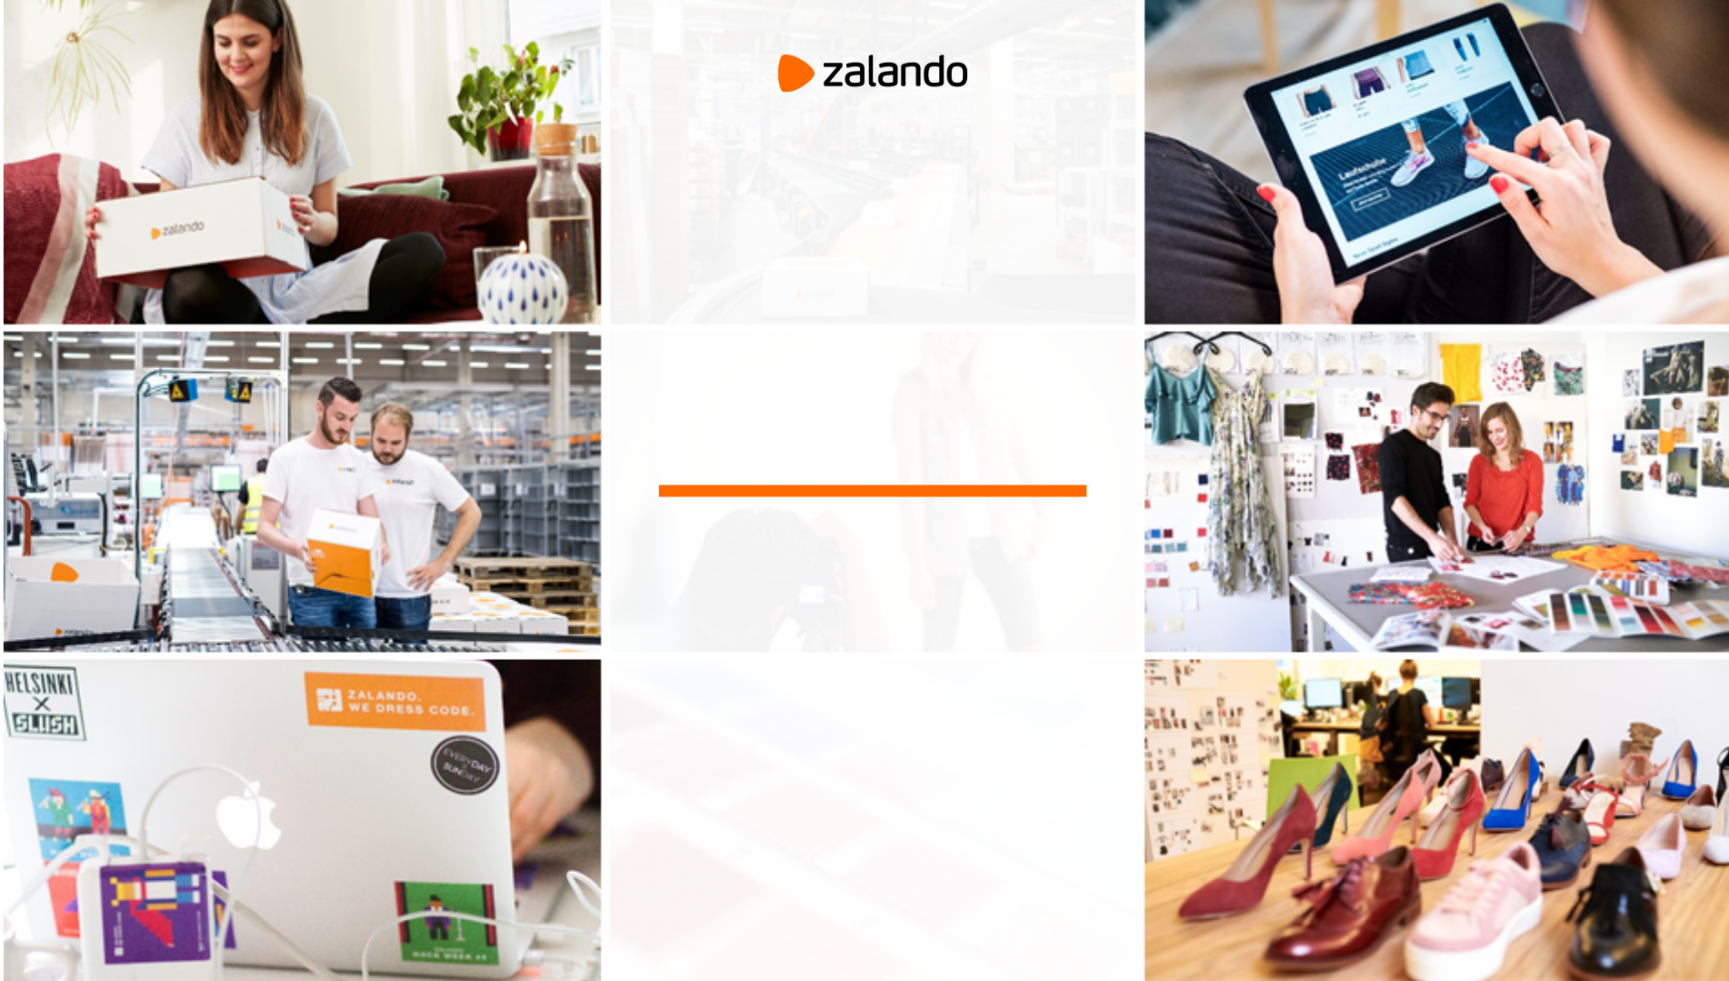
\includegraphics[width=\paperwidth]{template_2.png}}%
  \fontsize{17pt}{18}\selectfont
  \maketitle
}

\AddToShipoutPictureBG{
  \AtPagemyUpperLeft{{
\includegraphics[width=2.0cm,keepaspectratio]{logo.png}}}
}%

\setbeamertemplate{background canvas}{
\begin{tikzpicture}
    \clip (0,0) rectangle (\paperwidth,\paperheight);
    \fill[color=orange] (4cm, \paperheight-6pt) rectangle (\paperwidth-4cm,\paperheight);
\end{tikzpicture}
}

\fontsize{17pt}{18}\selectfont

\begin{frame}
    \frametitle{}
    \begin{center}
        \begin{itemize}[label={\MVRightarrow}]
            \item CPU
            \item CPU cache
            \item Storage IO
            \item Network
            \item Memory
            \item Hugetlb
        \end{itemize}

    \end{center}
\end{frame}

\begin{frame}
    \frametitle{}
    \begin{center}
        container = cgroup + namespace
    \end{center}
\end{frame}

\begin{frame}
    \frametitle{}
    \begin{center}

    \begin{tikzpicture}[
        scale=0.8,
        every node/.style={draw=black!70,fill=red!30,rounded corners,thick,anchor=west, minimum width=4cm,transform shape, blur shadow={shadow blur steps=5,shadow blur extra rounding=1.3pt}},
        inactive/.style={fill=gray!30},
        to/.style={->,>=stealth',shorten >=1pt,semithick,font=\sffamily\footnotesize},
        ]
      \node [circle, fill=yellow!20, minimum width=1cm] (cgroup-v1) {cg v1};
      \node [below=.5cm of cgroup-v1] (cpu) {cpu};
      \node [inactive, left=.5cm of cpu] (systemd) {systemd};
      \node [inactive, right=.5cm of cpu] (memory) {memory};
      \node [below=.5cm of cpu] (k8s) {k8s};
      \node [below=.5cm of k8s] (guaranteed) {guaranteed};
      \node [inactive, right=.5cm of guaranteed] (burstable) {burstable};
      \node [inactive, left=.5cm of guaranteed] (bestefforts) {bestefforts};
      \node [below=.5cm of guaranteed] (pause) {pause};
      \node [below=.5cm of pause] (app) {app};

      \draw[to] (cgroup-v1) -- (cpu);
      \draw[to] (cgroup-v1) -- (memory);
      \draw[to] (cgroup-v1) -- (systemd);
      \draw[to] (cpu) -- (k8s);
      \draw[to] (k8s) -- (guaranteed);
      \draw[to] (k8s) -- (bestefforts);
      \draw[to] (k8s) -- (burstable);
      \draw[to] (guaranteed) -- (pause);
      \draw[to] (pause) -- (app);
    \end{tikzpicture}

    \end{center}
\end{frame}

\begin{frame}
    \frametitle{}
    \begin{center}
    \textbf{CPU}

        \begin{itemize}[]
            \item directly manageable
            \item requests $\to$ cpu.share
            \item limits $\to$ cpu.cfs\_period \& cpu.cfs\_quota\_us
        \end{itemize}

    \end{center}
\end{frame}

\begin{frame}
    \frametitle{}
    \begin{center}
    \textbf{Share}

        \vspace{1.0cm}
        \only<1>{
            \begin{tikzpicture}
                \draw[
                    line width=0.5mm,
                    fill=red!30
                ] (0.0,0.0) rectangle (4.0,2.0) node[pos=.5] {\textbf{C1}};

                \draw[
                    line width=0.5mm,
                    fill=blue!30
                ] (4.0,0.0) rectangle (8.0,2.0) node[pos=.5] {\textbf{C2}};

            \end{tikzpicture}
        }

        \only<2>{
            \begin{tikzpicture}

                \draw[
                    line width=0.5mm,
                    fill=red!30
                ] (0.0,0.0) rectangle (2.0,2.0) node[pos=.5] {\textbf{C1}};

                \draw[
                    line width=0.5mm,
                    fill=blue!30
                ] (2.0,0.0) rectangle (4.0,2.0) node[pos=.5] {\textbf{C2}};

                \draw[
                    line width=0.5mm,
                    fill=green!30
                ] (4.0,0.0) rectangle (6.0,2.0) node[pos=.5] {\textbf{C3}};

                \draw[
                    line width=0.5mm,
                    fill=gray!30
                ] (6.0,0.0) rectangle (8.0,2.0) node[pos=.5] {\textbf{C4}};

            \end{tikzpicture}
        }

    \end{center}
\end{frame}

\begin{frame}
    \frametitle{}
    \begin{center}
    \textbf{Bandwidth}

        \vspace{1.0cm}
        \only<1>{
            \begin{tikzpicture}
                \draw[
                    line width=0.5mm,
                    fill=red!30
                ] (0.0,0.0) rectangle (2.0,2.0) node[pos=.5] {\textbf{C1}};

                \draw[
                    line width=0.5mm,
                    fill=blue!30
                ] (2.0,0.0) rectangle (4.0,2.0) node[pos=.5] {\textbf{C2}};

                \draw[
                    line width=0.5mm,
                    dashed
                ] (4.0,0.0) rectangle (8.0,2.0) node[pos=.5] {};

            \end{tikzpicture}
        }

        \only<2>{
            \begin{tikzpicture}

                \draw[
                    line width=0.5mm,
                    fill=red!30
                ] (0.0,0.0) rectangle (2.0,2.0) node[pos=.5] {\textbf{C1}};

                \draw[
                    line width=0.5mm,
                    fill=blue!30
                ] (2.0,0.0) rectangle (4.0,2.0) node[pos=.5] {\textbf{C2}};

                \draw[
                    line width=0.5mm,
                    fill=green!30
                ] (4.0,0.0) rectangle (6.0,2.0) node[pos=.5] {\textbf{C3}};

                \draw[
                    line width=0.5mm,
                    fill=gray!30
                ] (6.0,0.0) rectangle (8.0,2.0) node[pos=.5] {\textbf{C4}};

            \end{tikzpicture}
        }

    \end{center}
\end{frame}

\begin{frame}[fragile]{}
    \frametitle{}
    \begin{center}
        \textbf{Bandwidth accounting}

        \begin{flushleft}
        \begin{minted}[fontsize=\LARGE]{bash}
# from /proc/sys/kernel/
sched_cfs_bandwidth_slice_us
# default=5ms
        \end{minted}
        \end{flushleft}

    \end{center}
\end{frame}

\begin{frame}[fragile]{}
    \frametitle{}
    \begin{center}
        \textbf{Allocatable}

        \begin{flushleft}
        \begin{minted}[fontsize=\normalsize]{bash}
Capacity:
 cpu:                         16
 hugepages-1Gi:               0
 hugepages-2Mi:               0
 memory:                      65947396Ki
Allocatable:
 cpu:                         15800m
 hugepages-1Gi:               0
 hugepages-2Mi:               0
 memory:                      65388292Ki
        \end{minted}
        \end{flushleft}

    \end{center}
\end{frame}

\begin{frame}[fragile]{}
    \frametitle{}
    \begin{center}
        \textbf{Exclusive CPU}

        \begin{itemize}[]
            \item cpu management policy
            \item kube-reserved
			\item guaranteed
			\item integer quantity
            \item cpuset.cpus
            \item cpuset.cpuset.cpu\_exclusive
            \item cpuset.mems ?
        \end{itemize}

    \end{center}
\end{frame}

\begin{frame}[fragile]{}
    \frametitle{}
    \begin{center}
        \textbf{Cache}

        \begin{flushleft}
		\begin{minted}[fontsize=\normalsize]{bash}
# COS1 4 cache ways, COS 2 next 8 cache ways
=> pqos -e "llc:1=0x000f;llc:2=0x0ff0;"
SOCKET 0 L3CA COS1 => MASK 0xf
SOCKET 0 L3CA COS2 => MASK 0xff0
Allocation configuration altered.
        \end{minted}
        \end{flushleft}

    \end{center}
\end{frame}

\begin{frame}[fragile]{}
    \frametitle{}
    \begin{center}
        \textbf{Cache}

        \begin{flushleft}
		\begin{minted}[fontsize=\normalsize]{bash}
=> pqos -s
L3CA COS definitions for Socket 0:
	L3CA COS0 => MASK 0xffff
	L3CA COS1 => MASK 0xf
	L3CA COS2 => MASK 0xff0
	L3CA COS3 => MASK 0xfff
Core information for socket 0:
	Core 0, L2ID 0, L3ID 0 => COS0
	Core 1, L2ID 1, L3ID 0 => COS0
	Core 2, L2ID 0, L3ID 0 => COS0
	Core 3, L2ID 1, L3ID 0 => COS0
        \end{minted}
        \end{flushleft}

    \end{center}
\end{frame}

\begin{frame}
    \frametitle{}
    \begin{center}
    \textbf{Memory}

        \begin{itemize}[]
            \item directly manageable
            \item requests $\not \to$ memory.soft\_limit\_in\_bytes
            \item limits $\to$ memory.limit\_in\_bytes (OOM)
            \item memory.kmem.limit\_in\_bytes
            \item best efforts (not everything is accounted)
        \end{itemize}

    \end{center}
\end{frame}

\begin{frame}[fragile]{}
    \frametitle{}
    \begin{center}
        \textbf{Memory reclaim}

        \begin{flushleft}
        \begin{minted}[fontsize=\normalsize]{bash}
# only under the memory pressure
root@k8s-node-2:/home/vagrant# ./page_reclaim.py
Attaching...
Listening...
Detaching...
[7382] postgres: 928K
[7138] postgres: 152K
[7136] postgres: 180K
[7468] postgres: 72M
[7464] postgres: 57M
[5451] postgres: 1M
        \end{minted}
        \end{flushleft}

    \end{center}
\end{frame}

\begin{frame}[fragile]{}
    \frametitle{}
    \begin{center}
        \textbf{Writeback (cgroup v1)}

        \begin{flushleft}
        \begin{minted}[fontsize=\normalsize]{c}
/* vmscan.c */
/* The normal page dirty throttling mechanism
 * in balance_dirty_pages() is completely broken
 * with the legacy memcg and direct stalling in
 * shrink_page_list() is used for throttling instead,
 * which lacks all the niceties such as fairness,
 * adaptive pausing, bandwidth proportional
 * allocation and configurability.
 */
static bool sane_reclaim(struct scan_control *sc)
        \end{minted}
        \end{flushleft}

    \end{center}
\end{frame}
\note{
    default hierarchy is from cgroup v2
}

\begin{frame}[fragile]{}
    \frametitle{}
    \begin{center}
        \textbf{Writeback monitoring}

        \begin{flushleft}
        \begin{minted}[fontsize=\normalsize]{bash}
=> perf record -e writeback:writeback_written
kworker/u8:1 5816.288044: nr_pages=101429
kworker/u8:1 5816.288129: nr_pages=9223372036854775789
kworker/u8:3 5817.312319: nr_pages=101457
        \end{minted}
        \end{flushleft}

    \end{center}
\end{frame}

\begin{frame}[fragile]{}
    \frametitle{}
    \begin{center}
        \textbf{Writeback monitoring}

        \begin{flushleft}
        \begin{minted}[fontsize=\normalsize]{bash}
# pgbench insert
=> ./io_timeouts.py -p bin/postgres
Attaching...
Listening...
Detaching...
[18335] END: MAX_SCHEDULE_TIMEOUT
[18333] END: MAX_SCHEDULE_TIMEOUT
[18331] END: MAX_SCHEDULE_TIMEOUT
[18318] truncate pgbench_history: MAX_SCHEDULE_TIMEOUT
        \end{minted}
        \end{flushleft}

    \end{center}
\end{frame}

\begin{frame}[fragile]{}
    \frametitle{}
    \begin{center}
        \textbf{Huge pages}

        \begin{itemize}[]
			\item directly manageable
            \item transparent vs classic
            \item isolation only per pod
			\item no soft limits or reclaim (SIGBUS)
			\item TLB misses are faster and less frequent
            \item memory leaks (but PG is good)
        \end{itemize}

    \end{center}
\end{frame}

\begin{frame}[fragile]{}
    \frametitle{}
    \begin{center}
        \textbf{Huge pages}

        \begin{flushleft}
		\begin{minted}[fontsize=\normalsize]{bash}
# huge_pages on
Samples: 832K of event 'dTLB-load-misses'
Event count (approx.): 640614445 : ~19% less
Samples: 736K of event 'dTLB-store-misses'
Event count (approx.): 72447300 : ~29% less

# huge_pages off
Samples: 894K of event 'dTLB-load-misses'
Event count (approx.): 784439650
Samples: 822K of event 'dTLB-store-misses'
Event count (approx.): 101471557
        \end{minted}
        \end{flushleft}

    \end{center}
\end{frame}

\begin{frame}[fragile]{}
    \frametitle{}
    \begin{center}
        \textbf{Storage IO}

        \begin{itemize}[]
            \item blkio.weight
            \item blkio.throttle.*
			\item Not used in K8S
			\item sane\_behavior
            \item cpuset.cpus
            \item cpuset.cpuset.cpu\_exclusive
            \item cpuset.mems ?
        \end{itemize}

    \end{center}
\end{frame}

\begin{frame}[fragile]{}
    \frametitle{}
    \begin{center}
        \textbf{IO scheduler}

        \begin{flushleft}
		\begin{minted}[fontsize=\LARGE]{bash}
=> cat /sys/block/xvdcj/queue/scheduler
[mq-deadline] kyber bfq none
        \end{minted}
        \end{flushleft}

    \end{center}
\end{frame}

\begin{frame}[fragile]{}
    \frametitle{}
    \begin{center}
        \textbf{IO scheduler}

        \begin{flushleft}
BFQ distributes the bandwidth of of the device among all processes according to
their weights, regardless of the device parameters and with any workload.
        \end{flushleft}

    \end{center}
\end{frame}

\begin{frame}[fragile]{}
    \frametitle{}
    \begin{center}
        \textbf{IO scheduler}

        \begin{flushleft}
The Kyber I/O scheduler is a low-overhead scheduler suitable for multiqueue and
other fast devices. Given target latencies for reads and synchronous writes, it
will self-tune queue depths to achieve that goal.
        \end{flushleft}

    \end{center}
\end{frame}

\begin{frame}[fragile]{}
    \frametitle{}
    \begin{center}
        \textbf{Network}

        \begin{itemize}[]
			\item not directly
            \item network class
            \item traffic control
        \end{itemize}

    \end{center}
\end{frame}

\begin{frame}[fragile]{}
    \frametitle{}
    \begin{center}
        \textbf{Kernel noise}

        \begin{itemize}[]
			\item Futex
            \item Compaction
            \item Readahead
            \item Filesystem
            \item ...
        \end{itemize}

    \end{center}
\end{frame}
\note {
    readahead for io congested cgroups is not happen
}

\fontsize{18pt}{18}\selectfont
\begin{frame}
  \vspace*{2.5cm}
  \begin{minipage}[b][\paperheight]{\textwidth}
  \begin{center}

      %\raggedright%
      \linespread{1.0}%
      \usebeamerfont{title}%
      \usebeamercolor[fg]{title}%
      \if@noSmallCapitals%
        Questions?
      \else%
        \scshape{\color{black} Questions?}%
      \fi%
      \vspace*{0.3em}

      \usebeamerfont{subtitle}%
      \fontsize{13pt}{14}\selectfont
      \usebeamercolor[fg]{subtitle}%
        \begin{itemize}[label={}]
            \item {\color{black} \github\ \href{github.com/erthalion}
                                               {\color{black}github.com/erthalion}}
            \item {\color{black} \twitter\ @erthalion}
            \item {\color{black} \email\ dmitrii.dolgov at zalando dot de}
            \item {\color{black} \email\ 9erthalion6 at gmail dot com}
        \end{itemize}
      \vspace*{2.5em}%

    \vfill
    \vspace*{2em}
  \end{center}
  \end{minipage}

\end{frame}

\end{document}
